% Baccalauréat malgache, série C, 2018 : corrigé.
\TCDBacAttribution{C}{2018}
\providecommand{\cm}{~\mathrm{cm}}
\providecommand{\dx}{~\mathrm{d}x}
\providecommand{\Courbe}{(\mathscr{C})}
\providecommand{\Plan}{(\mathscr{P})}
\providecommand{\mes}[2]{\mathrm{mes}\left( \widehat{ \overrightarrow{#1} ; \overrightarrow{#2} } \right)}
\providecommand{\Angl}[2]{\left( \overrightarrow{#1} ; \overrightarrow{#2} \right)}
%
%%%%%%%%%%%%%%%%%%%%%%%%%%%%%%%%%%%%%%%%%%%%%%%%%%%%%%%%%%%%%%%%%%%%%%%%%%%%%%%%%%%%%%%%%%%%%%%%%%%%%%%%%%%%%%%%%%%%%%%%%%%%%%%%
\noindent \underline{\textsc{\textbf{Exercice}}} (4 points)
\begin{description}
	\item[I. Arithmétique :]
	\begin{enumerate}
		\item
		\begin{enumerate}
			\item \vln{$17$ divise $20A$ :}
				$20A = 4 \times 5 \times 3 \times 5^{2n-1} + 4 \times 5 \times 2^{3n-2} = 12 \times 5^{2n} + 5 \times 2^{3n} = 12 \times 25^n + 5 \times 8^n$.
				Or $25 = 17 + 8 \equiv 8 \pmod{17}$, donc $20A \equiv 12 \times 8^n + 5 \times 8^n = 17 \times 8^n \equiv 0 \pmod{17}$.
				\par\noindent\ansbox{$17$ divise $20A$.}
			\item \vln{$17$ divise $A$ :}
				$17$ est premier et ne divise pas $20$, donc $\pgcd{17}{20} = 1$ ; d'après le théorème de Gauss, $17 \mid 20A$ entraîne
				\par\noindent\ansbox{$17$ divise $A$.}
		\end{enumerate}
		\item \vln{Base $n$ :}
			$B = 3 \times 64 + 1 \times 16 + 2 \times 4 + 2 = 218$, et $B = 4n^2 + 3n + 1$ avec $n \geq 5$ (chiffre $4$).
			$4n^2 + 3n - 217 = 0$ : discriminant $9 + 3472 = 3481 = 59^2$, racines $\frac{-3 + 59}{8} = 7$ et $-\frac{31}{4}$.
			\par\noindent\ansbox{$n = 7$} ($4 \times 49 + 21 + 1 = 218$).
		\item \vln{Entiers $a$ et $b$ :}
			$a = 18a'$, $b = 18b'$ avec $\pgcd{a'}{b'} = 1$ ; $a^2 - b^2 = 324(a'^2 - b'^2) = 2916$ donne $(a' - b')(a' + b') = 9$, avec $0 < a' - b' < a' + b'$ (car $b' \geq 1$).
			Donc $a' - b' = 1$ et $a' + b' = 9$ : $a' = 5$, $b' = 4$, premiers entre eux.
			\par\noindent\ansbox{$a = 90$ et $b = 72$} ($8100 - 5184 = 2916$).
	\end{enumerate}
	\item[II. Probabilité :] L'urne contient $2n + n + 3 = 3n + 3$ jetons.
	\begin{enumerate}
		\item
		\begin{enumerate}
			\item \vln{$P(A)$ :}
				Le premier jeton est tiré au hasard parmi $3n + 3$ : \par\noindent\ansbox{$P(A) = \frac{2n}{3n + 3}$.}
			\item \vln{Limite :}
				\ansbox{$\lim_{n\to+\infty} P(A) = \frac{2}{3}$.}
		\end{enumerate}
		\item
		\begin{enumerate}
			\item \vln{$P(B)$ :}
				\ansbox{$P(B) = \frac{n + 3}{3n + 3}$.}
			\item \vln{Limite :}
				\ansbox{$\lim_{n\to+\infty} P(B) = \frac{1}{3}$.}
		\end{enumerate}
	\end{enumerate}
\end{description}
%%%%%%%%%%%%%%%%%%%%%%%%%%%%%%%%%%%%%%%%%%%%%%%%%%%%%%%%%%%%%%%%%%%%%%%%%%%%%%%%%%%%%%%%%%%%%%%%%%%%%%%%%%%%%%%%%%%%%%%%%%%%%%%%
\noindent \underline{\textsc{\textbf{PROBLEME I}}} (7 points) \newline
$AB = 2\cm$, $BC = 4\cm$, donc $AC = \sqrt{16 - 4} = 2\sqrt{3}\cm$ et $\widehat{ABC} = \frac{\pi}{3}$ ($\cos\widehat{ABC} = \frac{1}{2}$).
\begin{center}
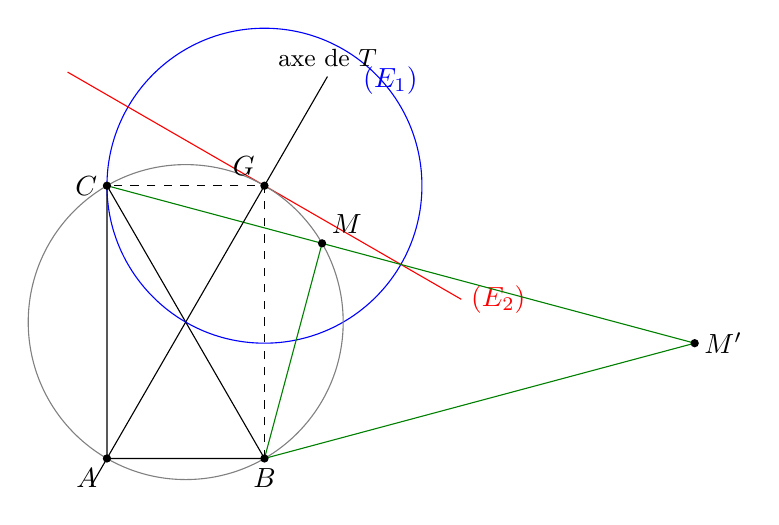
\begin{tikzpicture}[scale=1]
	\coordinate (A) at (0,0); \coordinate (B) at (2,0); \coordinate (C) at (0,3.464); \coordinate (G) at (2,3.464);
	\coordinate (M) at (2.732,2.732); \coordinate (Mp) at (7.464,1.464);
	\draw (A) -- (B) -- (C) -- cycle;
	\draw[dashed] (B) -- (G) -- (C);
	\draw[blue] (G) circle (2);
	\draw[red] (-0.5,4.907) -- (4.5,2.021) node[right] {$(E_2)$};
	\draw[gray] (1,1.732) circle (2);
	\draw[green!50!black] (C) -- (Mp) -- (B) -- (M);
	\draw[thin] (-0.2,-0.346) -- (2.8,4.85) node[above] {\small axe de $T$};
	\foreach \P/\L/\pos in {A/A/below left,B/B/below,C/C/left,G/G/above left,M/M/above right,Mp/M'/right}
		\fill (\P) circle (1.5pt) node[\pos] {$\L$};
	\node[blue] at (3.6,4.8) {$(E_1)$};
\end{tikzpicture}
\end{center}
\begin{description}
	\item[I. ]
	\begin{enumerate}
		\item Le triangle est construit ci-dessus (en vraie grandeur).
		\item
		\begin{enumerate}
			\item \vln{Point $G$ :}
				La somme des poids vaut $1$ ; $\overrightarrow{AG} = \overrightarrow{AB} + \overrightarrow{AC}$.
				\par\noindent\ansbox{$G$ est le quatrième sommet du rectangle $ABGC$.}
			\item \vln{Ensemble $(E_1)$ :}
				Leibniz : $-MA^2 + MB^2 + MC^2 = MG^2 - GA^2 + GB^2 + GC^2$ avec $GA = BC = 4$, $GB = AC = 2\sqrt{3}$, $GC = AB = 2$ :
				la constante vaut $-16 + 12 + 4 = 0$. La condition devient $MG^2 = 4$.
				\par\noindent\ansbox{$(E_1)$ est le cercle de centre $G$ et de rayon $2\cm$.}
			\item \vln{Vecteur constant :}
				\textit{Tel qu'il est écrit, le vecteur $-\overrightarrow{MA} + \overrightarrow{MB} + \overrightarrow{MC}$ (somme des coefficients $1$) vaut $\overrightarrow{MG}$ et n'est pas constant ;
				le vecteur constant est $-2\overrightarrow{MA} + \overrightarrow{MB} + \overrightarrow{MC}$ (somme des coefficients nulle), qui apparaît en (d).}
				$-2\overrightarrow{MA} + \overrightarrow{MB} + \overrightarrow{MC} = -2\overrightarrow{MA} + \left(\overrightarrow{MA} + \overrightarrow{AB}\right) + \left(\overrightarrow{MA} + \overrightarrow{AC}\right)$, donc
				\par\noindent\ansbox{$-2\overrightarrow{MA} + \overrightarrow{MB} + \overrightarrow{MC} = \overrightarrow{AB} + \overrightarrow{AC} = \overrightarrow{AG}$ pour tout $M$.}
			\item \vln{Ensemble $(E_2)$ :}
				La condition s'écrit $\overrightarrow{AG} \cdot \overrightarrow{MG} = 0$.
				\par\noindent\ansbox{$(E_2)$ est la droite passant par $G$ et perpendiculaire à $(AG)$}
				(la tangente en $G$ au cercle de centre $A$ passant par $G$) ; elle est tracée sur la figure.
		\end{enumerate}
	\end{enumerate}
	\item[II. ]
	\begin{enumerate}
		\item \vln{Rapport et angle de $S$ :}
			$S(B) = B$, $S(A) = C$ : rapport $\frac{BC}{BA} = 2$, angle $\Angl{BA}{BC}$. Le triangle $ABC$ est direct ($\Angl{AB}{AC} = \frac{\pi}{2}$), donc $\Angl{BA}{BC} = -\frac{\pi}{3}$.
			\par\noindent\ansbox{$S$ : centre $B$, rapport $2$, angle $-\frac{\pi}{3}$.}
		\item
		\begin{enumerate}
			\item Les points $M$ et $M'$ sont placés sur la figure (exemple).
			\item \vln{$S(M) = M'$ :}
				Soit $M_1 = S(M)$. La similitude $S$ transforme le triangle $BAC$, rectangle en $A$, en $BMM_1$ : on a $BM_1 = 2BM$ et
				$\Angl{MB}{MM_1} = \Angl{AB}{AC} = \frac{\pi}{2}$.
				$M$ est sur le cercle de diamètre $[BC]$, sur l'arc qui ne contient pas $A$ : $(MB) \perp (MC)$ et, $A$ et $M$ étant de part et d'autre de $(BC)$,
				$\Angl{MB}{MC} = -\Angl{AB}{AC} = -\frac{\pi}{2}$.
				Donc $\overrightarrow{MM_1}$ et $\overrightarrow{MC}$ sont colinéaires et de sens contraires : $M_1$ est sur la droite $(CM)$, au-delà de $M$ ;
				avec $BM_1 = 2BM$, c'est le point $M'$ de l'énoncé.
				\par\noindent\ansbox{$S(M) = M'$.}
		\end{enumerate}
	\end{enumerate}
	\item[III. ] Dans le repère $(A;\vec{u},\vec{v})$, l'unité est $1\cm$.
	\begin{enumerate}
		\item
		\begin{enumerate}
			\item \vln{Affixes :}
				\ansbox{$z_B = 2$, $z_C = 2\sqrt{3}\,i$, $z_G = 2 + 2\sqrt{3}\,i$.}
			\item \vln{Expression de $S$ :}
				$z' = \alpha z + \beta$ avec $2 = 2\alpha + \beta$ ($B$ invariant) et $2\sqrt{3}\,i = \beta$ ($S(A) = C$) ; d'où $\alpha = 1 - i\sqrt{3}$.
				\par\noindent\ansbox{$S : z' = \left(1 - i\sqrt{3}\right)z + 2\sqrt{3}\,i$.}
			\item \vln{Éléments caractéristiques :}
				$1 - i\sqrt{3} = 2\expo{-i\frac{\pi}{3}}$ et le point invariant est $\frac{2\sqrt{3}\,i}{1 - (1 - i\sqrt{3})} = 2 = z_B$.
				\par\noindent\ansbox{$S$ : centre $B$, rapport $2$, angle $-\frac{\pi}{3}$.}
		\end{enumerate}
		\item Notons $a = -1 + i\sqrt{3}$ et $b = -2 - 2i\sqrt{3}$.
		\begin{enumerate}
			\item \vln{Nature de $T$ :}
				$T$ est de la forme $z' = a\bar{z} + b$ avec $|a| = \sqrt{1 + 3} = 2 \neq 1$.
				\par\noindent\ansbox{$T$ est une similitude indirecte de rapport $2$.}
			\item \vln{Éléments caractéristiques :}
				Centre $\Omega(x;y)$ : $x + iy = (-1 + i\sqrt{3})(x - iy) - 2 - 2i\sqrt{3} = (-x + \sqrt{3}\,y - 2) + i(y + \sqrt{3}\,x - 2\sqrt{3})$.
				La partie imaginaire donne $\sqrt{3}\,x = 2\sqrt{3}$, $x = 2$ ; la partie réelle, $2x = \sqrt{3}\,y - 2$, $y = 2\sqrt{3}$ : $\Omega = G$.
				On vérifie alors $z' - z_G = a\,\overline{(z - z_G)}$ (car $a\,\overline{z_G} = 4 + 4\sqrt{3}\,i$ et $z_G - a\overline{z_G} = b$).
				$a = 2\expo{i\frac{2\pi}{3}}$ ; l'axe est la droite passant par $G$ dirigée par $\expo{i\frac{\pi}{3}}$ (car $\expo{i\frac{2\pi}{3}}\,\overline{\expo{i\frac{\pi}{3}}} = \expo{i\frac{\pi}{3}}$),
				c'est-à-dire la droite $y = \sqrt{3}\,x$, qui passe par $A$ et $G$.
				\par\noindent\ansbox{$T$ : similitude indirecte de centre $G$, de rapport $2$ et d'axe $(AG)$.}
		\end{enumerate}
	\end{enumerate}
\end{description}
%%%%%%%%%%%%%%%%%%%%%%%%%%%%%%%%%%%%%%%%%%%%%%%%%%%%%%%%%%%%%%%%%%%%%%%%%%%%%%%%%%%%%%%%%%%%%%%%%%%%%%%%%%%%%%%%%%%%%%%%%%%%%%%%
\noindent \underline{\textsc{\textbf{PROBLEME II}}} (9 points)
\begin{description}
	\item[Partie A.]
	\begin{enumerate}
		\item
		\begin{enumerate}
			\item \vln{Variations de $g$ :}
				$g'(x) = \frac{(x+1) - x}{(x+1)^2} - \frac{1}{x+1} = \frac{1 - (x+1)}{(x+1)^2} = -\frac{x}{(x+1)^2} \leq 0$ (nul seulement en $0$).
				\par\noindent\ansbox{$g$ est strictement décroissante sur $[0;+\infty[$, avec $g(0) = 0$.}
			\item \vln{Signe :}
				\ansbox{$g(x) < 0$ pour tout $x > 0$.}
		\end{enumerate}
		\item
		\begin{enumerate}
			\item \vln{Variations de $h$ :}
				$h'(x) = \frac{1}{x+1} - 1 + x - x^2 = \frac{1 - (x+1) + x(x+1) - x^2(x+1)}{x+1} = -\frac{x^3}{x+1} \leq 0$.
				\par\noindent\ansbox{$h$ est décroissante sur $[0;+\infty[$, avec $h(0) = 0$.}
			\item \vln{Signe :}
				\ansbox{$h(x) \leq 0$ pour tout $x \geq 0$.}
			\item \vln{Minoration :}
				$k(x) = \ln(x+1) - x + \frac{x^2}{2}$ : $k'(x) = \frac{1}{x+1} - 1 + x = \frac{x^2}{x+1} \geq 0$, $k(0) = 0$, donc
				\par\noindent\ansbox{$\ln(x+1) - x + \frac{x^2}{2} \geq 0$ pour $x \geq 0$.}
			\item \vln{Encadrement :}
				D'après (c) et (b) : $-\frac{x^2}{2} \leq \ln(x+1) - x \leq -\frac{x^2}{2} + \frac{x^3}{3}$ ; on divise par $x^2 > 0$ :
				\par\noindent\ansbox{$-\frac{1}{2} \leq \frac{\ln(x+1) - x}{x^2} \leq -\frac{1}{2} + \frac{x}{3}$ pour $x > 0$.}
			\item \vln{Limite :}
				$\frac{\frac{\ln(x+1)}{x} - 1}{x} = \frac{\ln(x+1) - x}{x^2}$ ; par les gendarmes,
				\par\noindent\ansbox{$\lim_{x\to 0^+}\frac{\frac{\ln(x+1)}{x} - 1}{x} = -\frac{1}{2}$.}
		\end{enumerate}
	\end{enumerate}
	\item[Partie B.]
	\begin{enumerate}
		\item \vln{Continuité en $0$ :}
			$\varphi(x) = \frac{\ln(x+1)}{x}$ pour $x > 0$ et $\varphi(0) = \frac{1}{f(0)} = 1$. Or $\lim_{x\to 0^+}\frac{\ln(1+x)}{x} = 1$ : $\varphi$ est continue à droite en $0$.
			Comme $\varphi(0) \neq 0$, $f = \frac{1}{\varphi}$ est aussi continue à droite en $0$.
			\par\noindent\ansbox{$f$ et $\varphi$ sont continues à droite en $0$.}
		\item
		\begin{enumerate}
			\item \vln{Taux d'accroissement :}
				$\frac{f(x) - f(0)}{x} = \frac{1}{x}\left(\frac{1}{\varphi(x)} - \frac{1}{\varphi(0)}\right)$, soit
				\par\noindent\ansbox{$\frac{f(x) - f(0)}{x} = -\frac{1}{\varphi(x)\,\varphi(0)} \cdot \frac{\varphi(x) - \varphi(0)}{x}$.}
			\item \vln{Limite :}
				$\frac{\varphi(x) - \varphi(0)}{x} = \frac{\frac{\ln(x+1)}{x} - 1}{x} \to -\frac{1}{2}$ (A.2.e) et $\varphi(x)\varphi(0) \to 1$ :
				\par\noindent\ansbox{$\lim_{x\to 0^+}\frac{f(x) - f(0)}{x} = \frac{1}{2}$ : $f$ est dérivable à droite en $0$ et $f'_d(0) = \frac{1}{2}$.}
		\end{enumerate}
		\item \vln{Limite en $+\infty$ :}
			$f(x) = \frac{x}{x+1}\cdot\frac{x+1}{\ln(x+1)}$ avec $\frac{x}{x+1} \to 1$ et $\frac{X}{\ln X} \to +\infty$ ($X = x + 1$).
			\par\noindent\ansbox{$\lim_{x\to+\infty} f(x) = +\infty$.}
		\item
		\begin{enumerate}
			\item \vln{Relation entre $f'$ et $g$ :}
				$f'(x) = \frac{\ln(x+1) - \frac{x}{x+1}}{\left(\ln(x+1)\right)^2}$, soit \par\noindent\ansbox{$f'(x) = -\frac{g(x)}{\left(\ln(x+1)\right)^2}$ pour $x > 0$.}
			\item \vln{Tableau :}
				D'après A.1.(b), $f'(x) > 0$ pour $x > 0$.
				\[
				\begin{array}{c|ccc}
					x & 0 & & +\infty \\ \hline
					f'(x) & \frac{1}{2} & + & \\ \hline
					 & & & +\infty \\
					f & & \nearrow & \\
					 & 1 & &
				\end{array}
				\]
		\end{enumerate}
		\item
		\begin{enumerate}
			\item \vln{Branche infinie :}
				$\frac{f(x)}{x} = \frac{1}{\ln(x+1)} \to 0$ et $f(x) \to +\infty$ : \par\noindent\ansbox{branche parabolique de direction $(Ox)$.}
			\item \vln{Tracé (unité $1\cm$) :}
				Demi-tangente en $(0;1)$ : $y = \frac{1}{2}x + 1$. Valeurs : $f(1) = \frac{1}{\ln 2} \approx 1{,}44$ ; $f(4) \approx 2{,}49$ ; $f(10) \approx 4{,}17$.
				\begin{center}
				\begin{tikzpicture}[x=1cm,y=1cm,>=stealth]
					\draw[->] (-0.3,0) -- (12.5,0) node[below] {$x$};
					\draw[->] (0,-0.3) -- (0,5) node[left] {$y$};
					\foreach \t in {1,...,12} \draw (\t,0.05) -- (\t,-0.05) node[below] {\small $\t$};
					\foreach \t in {1,...,4} \draw (0.05,\t) -- (-0.05,\t) node[left] {\small $\t$};
					\draw[red] (0,1) -- (3,2.5);
					\draw[blue,thick] (0,1) -- plot[domain=0.001:12.2,samples=120] (\x,{\x/ln(\x+1)});
					\node[blue] at (10,4.6) {$\Courbe$};
				\end{tikzpicture}
				\end{center}
		\end{enumerate}
	\end{enumerate}
	\item[Partie C.]
	\begin{enumerate}
		\item \vln{Encadrement de $\frac{1}{1+t}$ :}
			Pour $t \in [0;1]$ : $1 + t \geq 1$ donne $\frac{1}{1+t} \leq 1$ ; et $(1 - t)(1 + t) = 1 - t^2 \leq 1$ donne $1 - t \leq \frac{1}{1+t}$.
			\par\noindent\ansbox{$1 - t \leq \frac{1}{1+t} \leq 1$.}
		\item \vln{Encadrement de $f$ :}
			Pour $x \in ]0;1]$, on intègre sur $[0;x]$ : $x - \frac{x^2}{2} \leq \ln(1 + x) \leq x$. Comme $x - \frac{x^2}{2} = \frac{x(2 - x)}{2} > 0$,
			en passant aux inverses puis en multipliant par $x > 0$ : $1 \leq \frac{x}{\ln(1+x)} \leq \frac{2}{2 - x}$. Pour $x = 0$ : $f(0) = 1 = \frac{2}{2}$.
			\par\noindent\ansbox{$1 \leq f(x) \leq \frac{2}{2 - x}$ pour tout $x \in [0;1]$.}
		\item \vln{Encadrement de l'intégrale :}
			$f$ est continue sur $[0;1]$ ; on intègre : $\int_0^1 \frac{2}{2 - x}\dx = \left[-2\ln(2 - x)\right]_0^1 = 2\ln 2$.
			\par\noindent\ansbox{$1 \leq \int_0^1 f(x)\dx \leq 2\ln 2$} (numériquement $\int_0^1 f \approx 1{,}23$ et $2\ln 2 \approx 1{,}39$).
	\end{enumerate}
\end{description}
